\documentclass{oblivoir}
\usepackage{graphicx} % Required for inserting images
\usepackage{verbatim}
\usepackage{graphicx}
\usepackage[a4paper, total={6in, 8in}]{geometry}
\hypersetup{
    colorlinks=true,
    linkcolor=blue
}

\title{HW11}
\author{C311054 박민서}
\date{2024년 11월 25일}

\begin{document}

\maketitle

\section{최단 경로 알고리즘}
다익스트라 알고리즘을 선택했다.
단일 시발점에서의 경로만 구하면 되고 음이 아닌 가중치를 갖기 때문이다.

\section{class 설계}
\begin{verbatim}
    class MatrixWGraph {
    	int node; //노드의 갯수
    	int** length; //두 역 사이 소요시간
    	bool* s; //방문 처리
    	pair<int, int>* dist; //first는 이전 노드번호 second는 소요시간
    	Station* stlist; //역의 배열. 인덱스값이 노드의 번호가 된다
    	int count; //stlist에 들어있는 원소의 갯수
    	vector<vector<int>> transfer; //이름이 같은 역들의 노드번호가 하나의 배열을 이룸.
    
    public:
    	MatrixWGraph(int);
    	void AddVertex(int, string, int, string);
    	void Dijkstra(int, string, int, string);
    	void PrintRoute(int, int);
    	void PrintTime(int);
    };
\end{verbatim}
노드는 호선과 이름이 다른 역마다 하나씩 부여했다.
즉 같은 역이라도 호선이 다르면 다른 노드로 취급한다.

length는 두 역 사이 소요시간, 다른 말로는 두 노드 사이의 가중치가 들어있는 이차원 배열의 포인터이다. length[i][j]로 노드 i와 노드 j 사이의 시간을 얻는다.

s는 노드의 방문여부를 저장하는 배열이다. s[i]가 true면 노드 i를 방문한 것이다.

dist[i]는 이전에 방문한 노드의 번호와 시작점에서 i 노드까지 걸리는 시간을 pair로 저장한다.

위와 같이 특정 노드에 대한 정보를 배열의 인덱스로 접근하려면 노드마다 0부터 node-1 사이의 번호를 갖고있어야 한다.
이를 위해서 모든 역의 정보를 배열로 저장해놓은 것이 stlist이다.
stlist[i]에는 특정 역(노드)의 호선과 이름이 저장되고 이 역은 노드 번호 i를 갖게 된다.
이 호선과 이름은 Station이라는 구조체로 묶었다.
\begin{verbatim}
    struct Station {
    	int num;
    	string name;
    	Station(int n = 0, string s = "") :num(n), name(s) {};
    };
\end{verbatim}

count는 stlist에 현재 들어있는 원소 갯수를 세기 위한 변수다. 새로운 노드는 stlist[count++]에 추가한다.

transfer는 환승역에 대한 정보를 저장하기 위해 만들었다.
이름은 같고 호선이 다른 역들의 노드번호가 하나의 벡터에 들어간다. 환승역이 여러개라면 이 벡터도 여러개가 되므로 이차원 벡터이다.

\section{그래프 구성}

\begin{verbatim}
    MatrixWGraph::MatrixWGraph(int n = 0) :node(n), count(0) {
    	length = new int* [n];
    	for (int i = 0; i < n; i++) {
    		length[i] = new int[n];
    		for (int j = 0; j < n; j++) {
    			length[i][j] = MAXLEN;
    		}
    		length[i][i] = 0;
    	}
    	s = new bool[n]();
    	dist = new pair<int,int>[n];
    	stlist = new Station[n];
    }
\end{verbatim}
main함수가 stations1.txt에서 읽은 노드 갯수를 MatrixWGraph 생성자에게 전달한다.
노드의 연결 정보가 들어오기 전 length의 초기값은 모든 두 노드에 대해 MAXLEN이고 자기자신에 대해서(length[i][i])는 0이다. 
\begin{verbatim}
    #define MAXLEN 45000
\end{verbatim}
MAXLEN은 헤더파일에서 위와 같이 정의하였다. 호선은 최대 9개, 각 호선의 역은 최대 100개이므로 최대 900개의 역이 있을 수 있고 이어진 역 사이의 시간은 최대 60초이므로 두 역 사이의 시간은 45000초를 넘을 수 없다.

\begin{verbatim}
    void MatrixWGraph::AddVertex(int num1, string name1, int num2, string name2) {

    	Station station1(num1, name1);
    	Station station2(num2, name2);
    
    	int p1 = -1; //station1의 인덱스값
    	int p2 = -1; //station2의 인덱스값
    	for (int i = 0; i < count; i++) {
    		if (stlist[i].num == station1.num && stlist[i].name == station1.name) {
    			p1 = i;
    		}
    		if (stlist[i].num == station2.num && stlist[i].name == station2.name) {
    			p2 = i;
    		}
    	}
    	if (p1 < 0) {
    		p1 = count;
    		stlist[count++] = station1;
    	}
    	if (p2 < 0) {
    		p2 = count;
    		stlist[count++] = station2;
    	}
    
    	if (station1.name == station2.name) { //환승역
    		for (int i = 0; i < transfer.size(); i++) {
    			if (stlist[transfer[i][0]].name == station1.name) {
    				bool b1 = false, b2 = false;
    				for (int j = 0; j < transfer[i].size(); j++) {
    					if (p1 != transfer[i][j]) {
    						length[p1][transfer[i][j]] = length[transfer[i][j]][p1] = 30;
    					}
    					else b1 = true;
    					if (p2 != transfer[i][j]) {
    						length[p2][transfer[i][j]] = length[transfer[i][j]][p2] = 30;
    					}
    					else b2 = true;
    				}
    				if (!b1) transfer[i].push_back(p1);
    				if (!b2) transfer[i].push_back(p2);
    				return;
    			}
    		}
    		transfer.push_back({ p1,p2 });
    		length[p1][p2] = length[p2][p1] = 30;
    	}
    	else {
    		length[p1][p2] = length[p2][p1] = 60;
    	}
    	
    }
\end{verbatim}

main함수에서 역의 연결정보를 전달받아 그래프를 구성하는 함수이다.

첫번째 for문에서는
stlist에 해당 역에 대한 정보가 이미 저장되어 있다면 p1,p2에 그 노드 번호를 할당한다. for문을 빠져나온 뒤에도 p1,p2의 값이 할당되지 않은 채 -1이라면 아직 stlist에 없는 노드라는 뜻이니 새로 추가해준다.

마지막 if문에서는 환승역을 처리한다.
이름이 같은 역에서 다른 호선으로 환승하는 경우 어떤 호선으로 환승하든지 환승시간은 항상 30초가 되어야 한다. 그래서 만약 이름이 같은 역의 연결 정보가 들어온 경우 transfer에서 그 역에 대한 배열을 찾고 그 배열의 다른 모든 원소에 대해 length를 30초로 설정한다. 두 역 중 하나만 transfer배열에 존재하는 경우도 있을 수 있으므로 transfer배열에서 해당 노드를 발견하지 못한 경우 추가해준다.
만약 해당 역에 대한 배열이 transfer에 존재하지 않는다면 새로운 배열로 추가해준다.
그리고 이름이 다른 역에 대해서는 else문에서 length를 60으로 넣어준다.

\section{결과 분석}
\subsection{역이 두 개인 경우}
a. 입력파일
\begin{verbatim}
    cat stations1.txt
    2
    1 a 1 b
\end{verbatim}
\begin{verbatim}
    cat input1.txt
    1 a
    1 b
\end{verbatim}
b. 출력
\begin{figure}[h]
    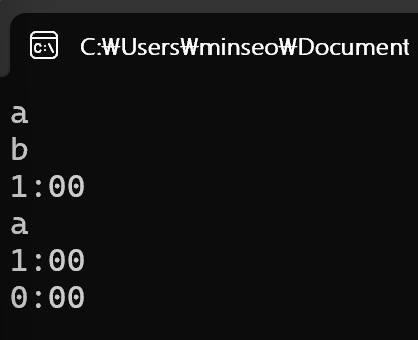
\includegraphics[width=0.3\linewidth]{result1.png}
\end{figure}

이 경우 중점은 a역과 b역 둘 다 가능하지만 중점을 찾는 코드가 다음과 같아서 도착점은 건너뛰기 때문에 a가 중점으로 출력되었다. 
\begin{verbatim}
    스택.push(도착점);
    while (스택.top() != 시작점){
        스택.push(스택.top()의 이전노드);
        
        //스택.top()이 중점인지 판단
        ...
    }
\end{verbatim}

\subsection{환승호선이 3개 이상인 경우}
a. 입력파일
\begin{verbatim}
    cat stations2.txt
    4
    1 a 2 a
    2 a 3 a
    3 a 3 b
\end{verbatim}
\begin{verbatim}
    cat input2.txt
    1 a
    3 b
\end{verbatim}
b. 출력
\begin{figure}[h]
    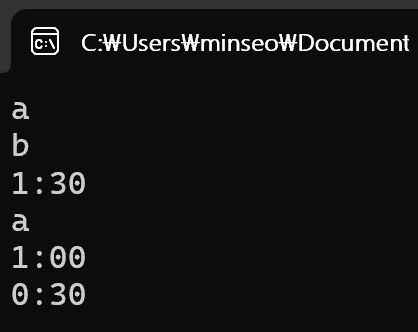
\includegraphics[width=0.3\linewidth]{result2.png}
\end{figure}

입력파일에는 1 a 3 a에 대한 정보가 없지만 환승역에 대한 시간처리를 따로 해주었기 때문에 1 a에서 3 a로 갈 때도 30초가 걸린다.

\subsection{최단 경로가 여러개인 경우}
a. 입력파일
\begin{verbatim}
    cat stations3.txt
    4
    1 a 2 a
    1 b 2 b
    1 a 1 b
    2 a 2 b
\end{verbatim}
\begin{verbatim}
    cat input3.txt
    1 a
    2 b
\end{verbatim}
b. 출력
\begin{figure}[h]
    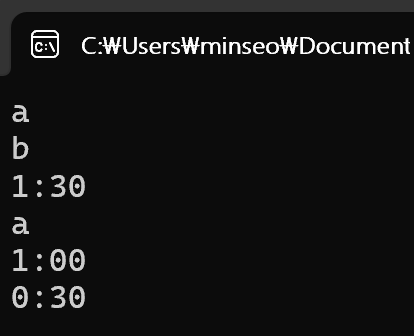
\includegraphics[width=0.3\linewidth]{result3.png}
\end{figure}

이 입력파일은 a역과 b역 사이에 1호선과 2호선이 모두 지나가는 경우다. a에서 환승하는 것과 b에서 환승하는 것 모두 최단 경로다. 출력 값을 보면 중점이 a이므로 여기서는 a에서 환승을 하는 경로가 나왔다. 이것은 최단경로가 여러개일 경우는 먼저 탐색된 경로가 출력되기 때문인데, 출발지에서의 소요시간이 짧은 노드를 우선 방문하기 때문에 1분이 걸리는 b로의 이동보다 30초가 걸리는 a에서의 환승 경로가 더 먼저 탐색된다.

\section{어려웠던 점}

\subsection{경로}
각 노드의 이전 노드를 저장해놓았기 때문에 경로를 출력하려면 도착점에서부터 이전노드를 계속 참조해서 시작점까지 역추적을 해야한다. 이는 경로의 반대방향이기때문에 경로를 정뱡향으로 출력하기위해 스택에 넣었다가 빼는 방법으로 출력했다.

\subsection{중점}
중점을 결정하기 위해 도착점까지의 소요시간의 절반에서 가장 가까운 값을 갖는 노드를 찾도록 했다.
스택에 노드를 넣는 과정에서 경로를 순회하므로 이 때 중점을 같이 찾도록 했다. 이 때 전체시간의 절반과 중점까지의 소요시간의 차이를 변수 midtime에 저장해놓고 이 값을 전체시간의 절반에 더한 값과 뺀 값이 중점까지의 소요시간이 된다.

\subsection{출력}
환승을 하는 경우에도 역의 이름은 한 번만 출력하기 때문에 이를 위해 이전 노드와 이름이 달라질 때까지 pop하도록 했다. 마지막 역에서 환승을 하는 경우도 똑같이 pop을 하면 범위를 넘어가는 인덱스를 참조하게 되므로 이전노드의 이름이 도착점의 이름과 같아지면 출력을 멈추도록 do-while문을 사용했다. 

\begin{verbatim}
    void MatrixWGraph::PrintRoute(int srcnum, int dstnum) {
    	stack<int> iroute;
    	iroute.push(dstnum);
    
    	int midnode = dstnum;
    	int midtime = MAXLEN;
    	while (iroute.top() != srcnum) {
    		iroute.push(dist[iroute.top()].first);
    
    		int temp = dist[iroute.top()].second - dist[dstnum].second / 2;
    		if (abs(temp) < midtime) {
    			midtime = abs(temp);
    			midnode = iroute.top();
    		}
    	}
    	int prenode = dstnum;
    	 do{
    		while (stlist[iroute.top()].name == stlist[prenode].name) {
    			iroute.pop();
    		}
    		cout << stlist[iroute.top()].name << endl;
    		prenode = iroute.top();
    		iroute.pop();
    	 } while (stlist[dstnum].name != stlist[prenode].name);
    	PrintTime(dist[dstnum].second);
    	cout << stlist[midnode].name << endl;
    
    	PrintTime(dist[dstnum].second / 2 + midtime);
    	PrintTime(dist[dstnum].second / 2 - midtime);
    
    }
\end{verbatim}

\subsection{시간표현}
소요시간을 초 단위로 저장해두었기 때문에 출력형식에 맞게 변환하는 과정이 필요하다. 이를 위한 함수를 따로 정의해 사용했다.
분은 초를 60으로 나눈 몫이고 초는 나머지에서 뒤의 0을 하나빼고 0을 다시 뒤에 붙여주면 0초일 때에도 00으로 두자릿수 표현이 된다. 이 연산은 소요시간이 모두 0으로 끝나기 때문에 가능하다.
\begin{verbatim}
    void MatrixWGraph::PrintTime(int time) {
    	cout << time / 60 << ':' << (time % 60) / 10 << 0 << endl;
    }
\end{verbatim}


\end{document}
